\documentclass[tikz,border=10pt]{standalone}
\usetikzlibrary{angles}
\begin{document}

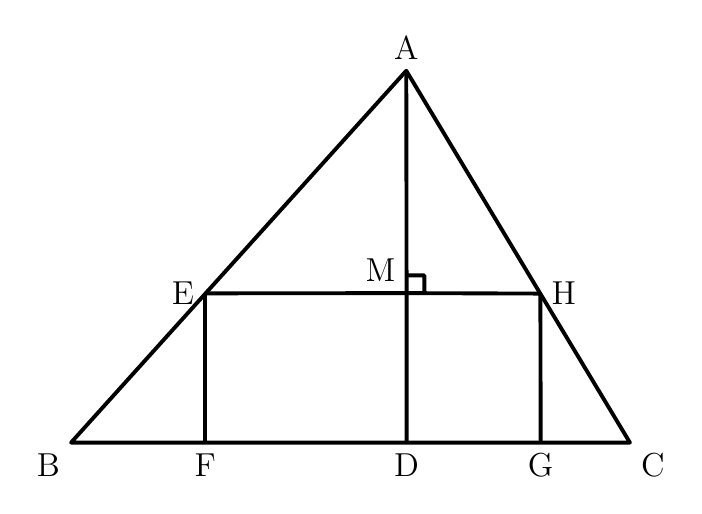
\begin{tikzpicture}[line join=round, line width=1.4pt, font=\fontsize{12}{14}\selectfont]
\coordinate (A) at (0.704,2.364);
\coordinate (B) at (-3.553,-2.358);
\coordinate (C) at (3.544,-2.358);
\coordinate (D) at (0.708,-2.358);
\coordinate (E) at (-1.850,-0.463);
\coordinate (G) at (2.411,-2.358);
\coordinate (H) at (2.407,-0.466);
\coordinate (M) at (0.708,-0.460);


\coordinate (F) at (-1.850,-2.358);


\draw (A) -- (B) -- (C) -- cycle;


\draw (A) -- (M) -- (D);
\draw (E) -- (M) -- (H);


\draw (E) -- (F);
\draw (H) -- (G);


\pic[draw, angle radius=0.226cm] {right angle=A--M--H};


\node[above] at (A) {$\mathrm{A}$};
\node[below left] at (B) {$\mathrm{B}$};
\node[below right] at (C) {$\mathrm{C}$};
\node[below] at (D) {$\mathrm{D}$};
\node[below] at (F) {$\mathrm{F}$};
\node[below] at (G) {$\mathrm{G}$};
\node[left] at (E) {$\mathrm{E}$};
\node[right] at (H) {$\mathrm{H}$};
\node[above left] at (M) {$\mathrm{M}$};
\end{tikzpicture}
\end{document}